\chapter{Fuzzy Set Theory}
This chapter draws upon foundational concepts and theoretical frameworks presented in \cite{FULLER1} and \cite{FULLER2}. 
\section*{Motivation}
Fuzzy sets were introduced by Zadeh...
\signal{the example of tall people, we want to model imprecision and why probability theory is not well suited for this. También pensar si voy a diferenciar entre incertidumbre epistemológica o aleatoria, o si eso lo meto cuando hable de possibility.}

\section{Fuzzy Sets}
\signal{Decir cómo a partir de ese concepto de partial membership llegamos a esto y cómo es una generalización de boolean membership de classical sets. Di también que con classical y crisp nos referimos a boolean sets y con fuzzy a los otros. Di que usas la xi para la boolean membership y mu para la fuzzy en general}

\begin{definition}[Fuzzy Set]
    Let $X\neq\emptyset$ a set. Then we define a \textbf{fuzzy set A in X}, i.e., $A \in \fuzzy{X}$ as:
    \[A=\{(x,\mu_A(x))\mid x\in X\}\]
    Where $\mu_A:X\longrightarrow [0,1]$ is the \textbf{membership function} and $X$ is the \textbf{domain} of the fuzzy set.
\end{definition}

\begin{remark}
     Both the fuzzy set and the membership function uniquely identify each other.
\end{remark}

\begin{notation}{Notation}
    We may use \( A(x) \equiv \mu_A(x) \) interchangeably.
\end{notation}

\begin{definition}[Support]
    Let $A \in \fuzzy{X}$. The set of non zero membership value elements is called the support:
    \[\textnormal{Supp}(A)=\{x\in X \mid A(x)>0\}\]
\end{definition}

\signal{
\begin{definition}[Normal Fuzzy Set]
    A fuzzy set is called \textbf{normal} if there exists $x\in X$ such that $A(x)=1$. Otherwise it is called \textbf{subnormal}.
\end{definition}
}
\begin{definition}[$\alpha$-cut]
    Let $\alpha \in [0,1]$, the $\alpha$-cut (also called $\alpha$-cut) of a fuzzy set \( A \in \fuzzy{X}\) is:
    \[
    [A]^\alpha =
    \begin{cases}
    \{x \in X \mid A(x)\geq \alpha\} & \text{if } \alpha > 0, \\
    \textnormal{cl}(\textnormal{Supp}(A)) & \text{if } \alpha = 0.
    \end{cases}
    \]
    where \textit{cl} denotes the closure.
\end{definition}

\signal{
    \begin{definition}[Extremes of the support]
        
    \end{definition}
}


\begin{definition}[Fuzzy Subset]
    Given the fuzzy sets $A, B \in \fuzzy{X}$ we say $A$ is a fuzzy subset of $B$ (and write $A \subseteq B$) if and only if $A(x)
    \leq B(x) \forall x \in X$.

    Analogously, $A$ and $B$ are equal if and only if $A(x)=B(x) \forall x \in X$, i.e., each of them is a subset of the other.
\end{definition}

\begin{example}
    Here are some examples of common fuzzy sets:
    \begin{itemize}
        \item \textbf{Empty Fuzzy Set in $X$:} such that $\emptyset(x)=0 \forall x \in X$.
        \item \textbf{Universal Fuzzy Set in $X$:} such that $X(x)=1  \forall x \in X$.
        \item \textbf{Fuzzy Point in $X$:} such that $P(x_0)=1 \land A(x)=0 \forall x \in X-\{x_0\}$
        \item \textbf{Fuzzy Number:} Usually defined as a fuzzy set in $\mathbb{R}$ with some desirable properties. Will be covered in Section \ref{sec:fuzzy_numbers}.
    \end{itemize}
\end{example}

\section{Operations over Fuzzy Sets and Fuzzy Relations}
\begin{notation}[label={not:OpsFS}]{Notation for variables in the current section}
    In this section, we use the variable \( x \) to represent time and \( y \) to represent distance.
  \end{notation}

\subsection{Union, Intersection and Complement of Fuzzy Sets}
\signal{say why we assign those properties to the union and intersection to generalize the ones from classical sets}
\begin{definition}[Triangular Norm]
    A mapping $T:[0,1]\times [0,1] \longrightarrow [0,1]$ that satisfies:
    \begin{enumerate}[(i)]\setlength{\itemindent}{2em}
      \item \textbf{Symmetricity:} $T(x,y) = T(y,x) \quad \oldforall x,y \in [0,1]$
      \item \textbf{Associativity:} $T(x,T(y,z)) = T(T(x,y),z) \quad \oldforall x,y,z \in [0,1]$
      \item \textbf{Monotonicity:} $T(x,y) \leq T(x',y') \quad \textnormal{if }x\leq x' \textnormal{ and } y\leq y' \quad \oldforall x,y,x',y' \in [0,1]$
      \item \textbf{One Identity:} $T(x,1) = T(1,x) = x \quad \oldforall x \in [0,1]$
    \end{enumerate}
    is called a triangular norm or t-norm. Defines the \textbf{intersection} of two fuzzy sets $A$ and $B$ on $X$ by giving the membership function as $(A \cup B) (x) = T(A(x),B(x)) \forall x \in X$ 
\end{definition}

\begin{definition}[Triangular Conorm]
  A mapping $S:[0,1]\times [0,1] \longrightarrow [0,1]$ that satisfies:
  \begin{enumerate}[(i)]\setlength{\itemindent}{2em}
    \item \textbf{Symmetricity:} $S(x,y) = S(y,x) \quad \oldforall x,y \in [0,1]$
    \item \textbf{Associativity:} $S(x,T(y,z)) = S(S(x,y),z) \quad \oldforall x,y,z \in [0,1]$
    \item \textbf{Monotonicity:} $S(x,y) \leq S(x',y') \quad \textnormal{if }x\leq x' \textnormal{ and } y\leq y' \quad \oldforall x,y,x',y' \in [0,1]$
    \item \textbf{Zero Identity:} $S(x,0) = S(0,x) = x \quad \oldforall x \in [0,1]$
  \end{enumerate}
  is called a triangular conorm or t-conorm. Defines the \textbf{union} of two fuzzy sets $A$ and $B$ on $X$ by giving the membership function as $(A \cap  B) (x) = S(A(x),B(x)) \forall x \in X$ 
    
\end{definition}

\begin{definition}[Complement]
    The complement of a fuzzy set $A\in \fuzzy{X}$ is another fuzzy set with membership function given by $^\lnot A(x) \coleq 1 - A(x) \forall x\in X$
\end{definition}

Notice that this definition of complement is consistent with the classical definition of complement but implies that an element might have \textbf{non-zero partial membership} to both a fuzzy set and its complement: Let $A$ be a fuzzy set on $X$ and $x \in X / A(x)\notin \{0,1\}$ then $\lnot A(x)= 1 - A(x) \notin \{0,1\}$.\\

This implies as well that the union of a fuzzy set and its complement is not the total set in general. Analogously, the intersection will not the empty set in general. Those two properties that hold in classical sets, are often called the \textbf{laws of excluded middle and of non-contradiction}, respectively.\\

However, there is a particular t-norm and t-conorm (named after Lukasiewicz) that does satisfy both laws. This will have implications for the derived logic that will be explained in section \ref{sec:fuzzy_logic}. \signal{is it the only one?}

\hspace{10em}$T_L(x,y)=\max\{x+y-1,0\},\, S_L(x,y)=\min\{1,x+y\}$\\

Another important property that classical union and intersection satisfy is De Morgan's Laws. For an arbitrary pair of t-norm and t-conorm they are not satisfied but by imposing it, we get that the t-norm induces a t-conorm and viceversa.

\begin{proposition}[Relationship between t-norm and t-conorm]
  Given a t-norm $T$, the t-conorm $S(a,b)\coleq 1 - T(1-a, 1-b)$, then the union and intersection defined by that pair satisfy the De Morgan's Laws.
\end{proposition}
\begin{remark}
  It is easy to see that the previous relation is equivalent to $T(a,b) = 1-S(1-a, 1-b)$ which can be obtained simply by substituting $a'=1-a$ and $b'=1-b$, i.e., working with the complementary fuzzy sets.
\end{remark}

\begin{proof}
  Let $x\in X$, $A$, $B$ be fuzzy sets over $X$ with $a \coleq A(x)$ and $b \coleq B(x)$\\

  $\quad \boxed{\text{not}(A \text{ or } B) = (\text{not } A) \text{ and } (\text{not } B)}$\\[0.5em]
  $\lnot S(a,b) = T(\lnot a, \lnot b) \implies 1 - S(a,b) = T(1-a, 1-b) \implies S(a,b) = 1 - T(1-a, 1-b)$\\

  $\quad \boxed{\text{not}(A \text{ and } B) = (\text{not } A) \text{ or } (\text{not } B)}$\\[0.5em]
  $\lnot T(a,b) = S(\lnot a, \lnot b) \implies 1 - T(a,b) = S(1-a, 1-b) \implies T(a,b) = 1 - S(1-a, 1-b)$

\end{proof}

\signal{
\begin{definition}[Archimedean t-norm]
  A continuous t-norm that satisfies $T(x,x)<x \forall x\in ]0,1[$ is called an archimedean t-norm.
\end{definition}

\begin{proposition}[Characterization of archimedean t-norms]
  For all archimedean t-norms there exists a continuous decreasing function $f:[0,1] \longrightarrow [0,\infty[$ with $f(1)=0$ such that: 
  \[ 
  T(x,y)= f^{-1}(\min\{f(x)+f(y), f(0)\}) \text{ where } f^{-1} =
  \begin{cases}
    f^{-1}(y) & \text{if } y\in [0,f(0) ]\\
    0 & \text{otherwise}
  \end{cases}
  \text{ is a pseudo-inverse}.
  \]
\end{proposition}
}

\signal{
\begin{definition}[Nilpotent t-norm]
  
\end{definition}}

\begin{definition}[Weaker t-norm]
  Given $T_1, T_2$ t-norms, then $T_1$ is weaker than $T_2$ $(T_1 \leq T_2)$ if $T_1(x,y)\leq T_2(x,y)\forall x,y\in [0,1]$.\\
  In that case, it is equivalent to say $T_2$ is stronger than $T_1$ $(T_2 \geq T_1)$

\end{definition}
\begin{remark}
  This defines a partial order relation in the set of t-norms.
\end{remark}
\signal{The weaker the t-norm, the stronger the associated s-norm? (not proved in Fuller)}

\signal{
There are many results like all t-norms are between the weak and the min, all t-conorms are between max and strong, or that min is the only t-norm that satisfies $T(a,a)=a$ (igual es por esto ultimo q se usa tanto. Qué implicaciones tiene que lukasiewicz no cumpla eso?)}

\signal{Tambien lo de que la T-norm e dsitributiva con max/sup sirve para justificar la definicion del producto cartesiano.}

\begin{example}
  \signal{Some examples of t-norms and t-conorms.}
\end{example}

\subsection{Fuzzy Relations}
\signal{Igual esto motivar la definición de relación con un ejemplo a estas alturas es pasarse?}

In the previous sections we have been working with a single domain denoted by $X$. Intuitively, it might be useful to think about the domain as the possible values of a property independently of the object that has that property. For example, we could say that for the property \textit{lenght} the domain is $\R^+\coleq
\{x\in\R \min x \geq 0\}$ and a person might have a \textit{height} defined in that domain (modeled as a fuzzy subset), although not all possible lengths values will be part of the support of a person's height since it is save to assume impossible to be 10 meters tall. If we were to look at the arm length, then we would have another subset of the lenghts. Treating each subset independently, doesn't allow to distinguish between the people of the same height with different arm lenght or viceversa. Therefore it is needed to a way to differentiate each unique combination of attributes. Notice that in this example, height and arm length have the same domain but for example hair color would have a different domain.\\

Mathematically, this is done with \textbf{relations} which are subsets of the cartesian product of the domains, so that each element is a unique possible combination of attributes, an ordered n-tuple. For simplicity, let us consider just the cartesian product of 2 sets since the general case can be obtained inductively. Again, the "fuzzy" part will be referred to how we generalize the membership values to the continuum.\\


\begin{definition}[Fuzzy Relation]
  Let $X\neq \emptyset \neq Y$ be classical sets. Then a fuzzy relation $R$ is a fuzzy set on $X\times Y$, i.e., $R\in \fuzzy{X\times Y}$. $R(x,y)$ will denote the degree of membership of $(x,y) \in R$
\end{definition}

\begin{remark}
  To formally extend the Cartesian product from two sets to \( n \) sets using induction, it is important to observe that it satisfies associativity up to a natural isomorphism, i.e., 
  \[
  (A\times B)\times C \cong A\times (B\times C).
  \]
\end{remark}

Before giving the definition of the fuzzy cartesian product, we need to first understand what the classical cartesian product is in terms of the membership function. When we define a cartesian product $A\times B$ as "\textit{all unique ordered pairs of elements from $A$ \textbf{and} $B$}", in terms of membership functions we are taking the intersection of membership to $A$ and membership to $B$. Therefore, generalizing that notion with a t-norm we get the following definition.

\begin{definition}[Fuzzy Cartesian Product]
  It is a fuzzy relation $A\times B \in \fuzzy{X\times Y}$ such that the membership function is given by:
  \[ 
  (A\times B)(x,y) = T(A(x), B(y)), \quad \forall (x,y) \in X\times Y
  \]
  where $T$ is a t-norm.
\end{definition}

To justify the definition of the membership function of a cartesian product of two fuzzy sets, let us first recall that in classical sets, we can retrieve the orginal subsets individually by taking the projection of the cartesian product. Given $R$ a relation on $X\times Y$ the projections are:

\[\Pi_X(R)=\{x \in X \mid \exists y \in Y \textnormal{ such that } (x,y) \in R\}\]
\[\Pi_Y(R)=\{y \in Y \mid \exists x \in X \textnormal{ such that } (x,y) \in R\}\]

Then, with the boolean membership, it can be expressed as well as:

\[\Pi_X(R)(x)=\sup\{R(x,y) \mid y\in Y\}=
\begin{cases}
  1 & \textnormal{if } \exists y \in Y \textnormal{ such that } (x,y) \in R \\
  0 & \textnormal{otherwise}
\end{cases}
\]
\[
  \Pi_Y(R)(y)=\sup\{R(x,y) \mid x\in X\}=
  \begin{cases}
    1 & \textnormal{if } \exists x \in X \textnormal{ such that } (x,y) \in R \\
    0 & \textnormal{otherwise}
  \end{cases}
\]

It is clear that in the case of having 2 possible values for the membership function, the above expresions are identical. The use of $\sup$ in the definition of the projection can be intuitively interpreted as the \textit{shadow} of the membership function of the cartesian product, as figure \ref{fig:class_cart_prod} illustrates. It is also desirable because then the following property holds for any classical \signal{(and fuzzy?)} cartesian product:\\
$$ 
\Pi_X(A\times B)=A \quad \textnormal{ and } \quad \Pi_Y(A\times B)=B \forall A\in X, \forall B \in Y
$$

\begin{figure}[ht]
  \centering
  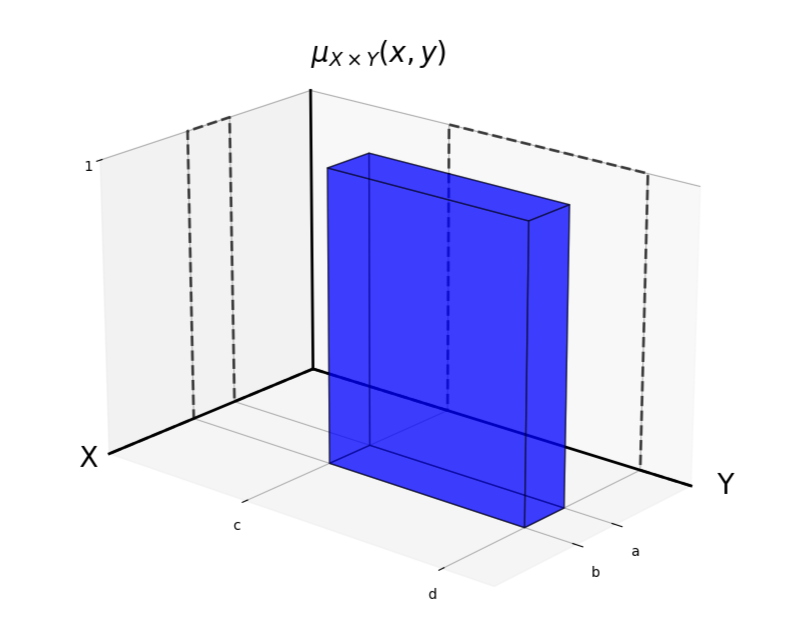
\includegraphics[width=0.65\textwidth]{ch1/figures/class_cart_prod.png}
  \caption{The blue volume represents the membership function of the cartesian product of two classical sets $X=[a,b]$ and $Y=[c,d]$ in $\R$. In the plane $y=0$ we have the projection that corresponds to the membership function of $X$ and analogously, the projection of $Y$ in the plane $x=0$.}
  \label{fig:class_cart_prod}
\end{figure}

Therefore, we define:

\begin{definition}[Projection of a fuzzy relation]
  The projection from fuzzy relations on $X\times Y$ onto the fuzzy sets on $X$ is the function:
  \[
    \begin{aligned}
      \Pi_X: \fuzzy{X\times Y} &\longrightarrow \fuzzy{X} \\
      R &\longmapsto \Pi_X(R)
    \end{aligned}
  \]
  where $\Pi_X(R)(x) = \sup_{y\in Y}\{R(x,y)\}\forall x \in X$
\end{definition}

Applying the definition of projection with the supremum to fuzzy sets, we have a way to retrieve the membership function of each fuzzy set given the membership function of a fuzzy cartesian product (figure \ref{fig:fuzzy_cart_prod}). \\






\begin{figure}[ht]
    \centering
    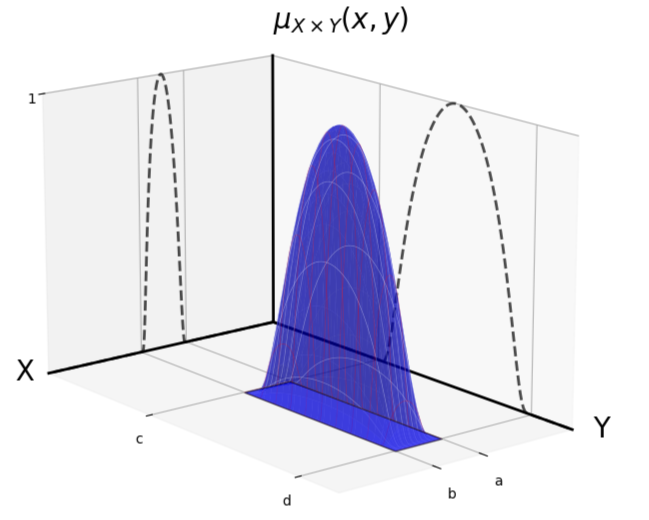
\includegraphics[width=0.65\textwidth]{ch1/figures/fuzzy_cart_prod.png}
    \caption{The blue volume represents the membership function of the cartesian product of two fuzzy sets $X$ and $Y$. In the plane $y=0$, we have the projection that corresponds to the membership function of $X$, and analogously, the projection of $Y$ in the plane $x=0$. The partial memberships illustrate how the fuzzy relations can vary across the domains.}
    \label{fig:fuzzy_cart_prod}
\end{figure}

\signal{Falta ver que que la proyección nos devuelve el fuzzy set original en los fuzzy cart prod.}

\subsubsection*{Composition of Fuzzy Sets}
\begin{notation}[label={not:compositionFS}]{Notation}
    Although Fuzzy Relations are Fuzzy Sets as well, we will often use the name distinction to denote whether the domain is a cartesian product or not.
  \end{notation}

% The definition of projection allows us to define a composition of fuzzy relations with a common domain. Intuitively, a composition is the projection into the uncommon domain of the intersection of each fuzzy relation.

% \begin{definition}[Composition of 2 Fuzzy Relations]
%     Let $R\in \fuzzy{X\times Y}$, $G \in \fuzzy{X\times Y}$ be 2 fuzzy relations with one of the sets of the domain in common. Then the composition is another fuzzy relation $R\circ G\in \fuzzy{X\times Z}$ (the non common sets of the domain) and the membership function is given by the projection of the cartesian product:
%     \[
%     (R \circ G) (x,z) = \Pi_{X\times Z}[T(R(x,y), G(y,z))] = \sup_{y\in Y}\{T(R(x,y), G(y,z))\}
%     \]
% \end{definition}

The concept of projection allows us to combine fuzzy relations sharing a common domain. Intuitively, composing two fuzzy relations involves intersecting their membership values (using a t-norm) and then projecting the result onto the domain where the relations do not overlap.

\begin{definition}[Composition of Two Fuzzy Relations]
    Let \( R \in \fuzzy{X \times Y} \) and \( G \in \fuzzy{Y \times Z} \) be fuzzy relations sharing the set \(Y\). Their composition \( R \circ G \) is the fuzzy relation in \(\fuzzy{X \times Z}\) defined by
    \[
    (R \circ G)(x,z) = \Pi_{X\times Z}\Bigl[\, T\bigl(R(x,y), G(y,z)\bigr) \Bigr] = \sup_{y\in Y}\, T\bigl(R(x,y), G(y,z)\bigr),
    \]
    where \(T\) is a t-norm acting as the fuzzy intersection.
\end{definition}

% This means that given three properties $X$, $Y$ and $Z$ and two fuzzy relation R from X to Y and another fuzzy relation from Y to Z, we have a way to induce a relation $R\circ G$ between X and Z.

% (add a diagram here)

Given three sets \(X\), \(Y\), and \(Z\), suppose we have a fuzzy relation \(R\) from \(X\) to \(Y\) and another fuzzy relation \(G\) from \(Y\) to \(Z\). Using the composition operation, we can derive a new fuzzy relation \(R \circ G\) that directly connects \(X\) to \(Z\).

\noindent
\begin{minipage}{0.7\textwidth}
In this diagram, the arrows represent fuzzy relations, with \(R\) mapping elements from \(X\) to \(Y\), \(G\) mapping from \(Y\) to \(Z\), and \(R \circ G\) representing the induced fuzzy relation between \(X\) and \(Z\) through composition.\\
\end{minipage}%
\begin{minipage}{0.3\textwidth}
  \begin{center}
    \begin{tikzcd}
      X \arrow[r, "R", leftrightarrow] & Y \arrow[r, "G", leftrightarrow] & Z \arrow[bend right=30, from=1-1, "R \circ G"', leftrightarrow]
      \end{tikzcd}
  \end{center}

\end{minipage}


We can define a the composition of a fuzzy set with a fuzzy relation in a completely analogous way. 

\begin{definition}[Composition of a Fuzzy Set and a Fuzzy Relation]
    Let \( A \in \fuzzy{X} \) be a fuzzy set on \(X\) and \( R \in \fuzzy{X \times Y} \) be a fuzzy relation between \(X\) and \(Y\). The composition \( A \circ R \in \fuzzy{Y} \) is defined by
    \[
    (A \circ R)(y) = \Pi_{Y}\Bigl[\, T\bigl( A(x), R(x,y) \bigr) \Bigr] = \sup_{x \in X}\, T\bigl( A(x), R(x,y) \bigr),
    \]
    where \(T\) is a t-norm.
\end{definition}



\subsection{Extension Principle}

Following a similar idea as in the definition of the composition of fuzzy sets, we can derive a way to generalize crisp functions \signal{(Hasta ahora lo he llamado classical en vez de crisp, tengo que explicarlo y elegir una notación uniforme)} to fuzzy sets.\\

Let's consider the crisp function $f:\,X \longrightarrow Y$ where $X$ and $Y$ are classical sets. And consider as well the fuzzy sets $A \in \fuzzy{X}$. Then $f$ induces the classical relation $R=\{(x,y)\in X\times Y \mid f(x)=y\}$. And we can also make this relation fuzzy by copying the membership function of $A$:
$$ \mu_R (x,y) = \mu_A (x) \forall (x,y)\in R$$
Now we can define $B\in\fuzzy{Y}$, the fuzzy image of $A$ under $f$, as the projection of this fuzzy relation:
$$\mu_B (y) = \Pi_Y (R) = \sup\{R(x,y)\mid x\in X\} = \sup\{\mu_A (x)\mid x\in X, \, f(x)= y\} = \sup_{x\in f^{-1}(y)}\{\mu_A(x)\}$$

This is called the (Zadeh's) extension principle and is the basis for building arithmetic for fuzzy numbers (see section \ref{sec:fuzzy_numbers}) and generalizing any crisp function to fuzzy sets: 

\begin{definition}[Zadeh's extension principle]
  Let $f: X \longrightarrow Y$ be a crisp function and $A\in \fuzzy{X}$ a fuzzy set on $X$. Then we can define $f(A)\in \fuzzy{Y}$ as:
  \[
  \mu_{f(A)}(y)\equiv f(A)(y) = 
  \begin{cases}
    \sup_{x\in f^{-1}(y)}A(x) & \textnormal{if } f^{-1}(y)\neq \emptyset\\
    0 & \textnormal{otherwise}
  \end{cases}
  \quad\quad\quad \textnormal{where } f^{-1}(y)=\{x\in X \mid f(x)=y\}
  \]
\end{definition}


\begin{remark}
  If $f$ is \textbf{injective} then for any $y \in \textnormal{Im}(f)$ there exists a unique $x \in X$ such that $f(x)=y$, and therefore $f^{-1}(y)=\{x\}$. Then the first case can be rewritten as, $f(A)(y) = A(f^{-1}(y))$ if $y \in \textnormal{Im}(f)$.
\end{remark}

It is important to highlight as well that this definition is straight forward generalization of set-valued functions where $f(A)= \{f(x)\mid x\in A\}$. In terms of boolean membership function:
$$\chi _{f(A)}(y)=\sup_{x\in f^{-1}(y)}\chi_A(x)$$

The definition above can be generalized to vector functions using the definition of fuzzy cartesian product, which requires us to take the intersection:

\begin{definition}[Sup-T extension principle]
  Let $f: X_1 \times \cdots \times X_n \longrightarrow Y$ be a crisp function and $A_1 \in \fuzzy{X_1}, \ldots, A_n \in \fuzzy{X_n}$ be fuzzy sets. Then we can define $f(A_1,\ldots,A_n)\in \fuzzy{Y}$ as:
  \[
  \mu_{f(A_1,\ldots,A_n)}(y)\equiv f(A_1,\ldots,A_n)(y) = 
  \begin{cases}
    \sup_{(x_1,\ldots,x_n)\in f^{-1}(y)} T(A_1(x_1),\ldots,A_n(x_n)) & \textnormal{if } f^{-1}(y)\neq \emptyset\\
    0 & \textnormal{otherwise}
  \end{cases}
  \]
  where $f^{-1}(y)=\{(x_1,\ldots,x_n)\in X_1\times\cdots\times X_n \mid f(x_1,\ldots,x_n)=y\}$ and $T$ is a t-norm.
\end{definition}

Which is again a generalization of vector set-valued functions where: $$f(A_1,\ldots,A_n)= \{f(x_1,\ldots,x_n)\mid x_i\in A_i\}$$
In terms of boolean membership function:
$$\chi _{f(A_1,\ldots,A_n)}(y)=\sup_{(x_1,\ldots,x_n)\in f^{-1}(y)}T(\chi_{A_1}(x_1),\ldots,\chi_{A_n}(x_n)) = \sup_{(x_1,\ldots,x_n)\in f^{-1}(y)}min\{\chi_{A_1}(x_1),\ldots,\chi_{A_n}(x_n)\}$$

Where we have used that every t-norm operates the same on boolean memberships. \signal{Debería haber puesto esto como un remark cuando presento la intersección y la unión.}
\section{Fuzzy Logic}\label{sec:fuzzy_logic}

Considering partial memberships and working with fuzzy sets has many implications for the logical framework that is derived from it. The field is vast and is best understood from the perspective of algebraic logic (see appendix \ref{app:alg_log}). However, this section only aims to very briefly introduce without proof some of the main results and concepts related to fuzzy logics: fuzzy implications, different fuzzy logics derived from t-norms and approximate reasoning.\\

In classical propositional logic\footnote{See appendix \ref{app:form_log} for a brief introduction to the concepts of formal logic}, there is a very straightforward relation between set-membership and truth values. It is the same to state \say{$x$ belongs to $A$} or \say{(it is true that) $x$ is $A$}. This direct correspondence extends to the fundamental operations of sets and logical connectives: stating that \say{$x$ belongs to the intersection of $A$ and $B$} (denoted $x \in A \cap B$) is equivalent to asserting that \say{$x$ is $A$ AND $x$ is $B$} (the logical conjunction $P_A(x) \land P_B(x)$ is true). The case for union $\cup$ and disjunction $\lor$ is analogous. Finally, the concept of an element $x$ belonging to the negation of set $A$ ($x \in \overline{A}$), meaning $x$ does not belong to $A$, directly mirrors logical negation ($\neg$). When working with fuzzy sets, we consider partial truth (degrees of truth as degrees of membership).\\

The implication connective is rooted in the residuation (or adjointness) property, which views implication $I$ ($A \Rightarrow B$, or "if $A$, then $B$") as a form of logical division: $A \land I \models B$ in logic (or $A \cap I \subseteq B$ in set theory). The goal is to find the weakest proposition (or largest set)\footnote{Intersection with a larger set $I$ is less restrictive respect to inclusion of sets. If intersection with the largest set is contained, intersection with any smaller set will also be contained.} $I$ such that combining $A$ with $I$ through conjunction (intersection) yields something at least as strong as (contained in) $B$. This largest $I$ satisfying the condition defines the implication $A \Rightarrow B$, internalizing the notion of logical consequence. Logical equivalence ($A \iff B$, or "$A$ if and only if $B$") occurs when both $A \Rightarrow B$ and $B \Rightarrow A$ hold. In set theory, this corresponds to mutual subset relations ($A \subseteq B$ and $B \subseteq A$), which can only be true when sets $A$ and $B$ are identical. Thus, logical equivalence between propositions directly corresponds to set equality.



\subsection{Fuzzy implications}
S-implications
R-implications
t-norm implications
\signal{$(\fuzzy{X},\cup , \cap , \lnot)$ is a complete, completely distributive, lattice with an involution. This extends the boolean algebra.}

\signal{The notion of equality is replaced by a graded relation (often measured via the biresiduum $\leftrightarrow$)}

\signal{Fuzzy description logics explained %https://www.umbertostraccia.it/cs/download/papers/KES09/KES09.pdf

The Lukasiewicz t-conorm is closely related to the basic binary operation of multi-valued
algebras. Additionally, t-norms and t-conorms form examples of aggregation operators. They
play a significant role in the axiomatic definition of the concept of triangular norm-based measure
and, in particular, of the concept of probability of fuzzy events; the Frank family of t-norms and
t-conorms plays a particular role [6]. 

%https://cake.fiu.edu/Publications/Ngan+al-18-LC.Logic_Connectives_of_Complex_Fuzzy_Sets_ROMJIST_downloaded.pdf 

It should be mentioned that t-norms overlap with copulas [3, 24]: commutative associative
copulas are t-norms; t-norms which satisfy the 1-Lipschitz condition are copulas. Some families
of t-norms are known as families of copulas under different names}

\signal{
    Lukasiewicz logic algebraic structure and formal implications thanks to the residual property.\\

    Gödel Logic uses 
    $a \otimes b = \min(a, b)$, which tends to produce conservative scores dominated by the weakest criterion. While useful for risk-averse scenarios, it fails to differentiate alternatives when all criteria are partially satisfied.

    Product Logic employs 
    $a \otimes b = a \cdot b$, amplifying the impact of low-scoring criteria. This can lead to premature elimination of alternatives with one poor attribute.

    Łukasiewicz Logic's additive t-norm balances compensation between criteria, allowing alternatives to offset weaknesses in one dimension with strengths in others—a critical feature for complex trade-off analysis.
}








\subsection{Approximate Reasoning and Pavelka-Style Completeness}

Classical deductive systems typically deal with absolute truth: premises are assumed to be fully true (truth value 1), and sound inference rules guarantee that conclusions are also fully true. However, in many real-world scenarios and in the spirit of fuzzy logic, we often reason with information that is only partially true or true to a certain degree. This leads to the field of **approximate reasoning**, where we are interested in the degree to which a conclusion follows from premises that themselves have degrees of truth.

A significant contribution to formalizing reasoning with degrees of truth was made by Jan Pavelka in the 1970s, particularly for logics related to Łukasiewicz logic. His work was later refined and integrated into the broader t-norm based framework by Hájek. The core idea is to extend a fuzzy logical system (like Łukasiewicz logic, denoted L) with rational truth constants $\bar{r}$ for every rational $r \in [0,1] \cap \mathbb{Q}$. A formula $(\bar{r} \rightarrow \phi)$ can then be interpreted as stating "$\phi$ is true to a degree at least $r$".

This framework allows for the definition of two key concepts for a given theory $T$ (a set of axioms, each potentially associated with a truth degree or assumed to be fully true):

\begin{itemize}
    \item \textbf{Truth Degree of $\phi$ over $T$}: $||\phi||_T = \inf\{e(\phi) \mid e \text{ is a model of } T\}$. This is the lowest degree to which $\phi$ is true in all models that satisfy the theory $T$.
    \item \textbf{Provability Degree of $\phi$ over $T$}: $|\phi|_T = \sup\{r \mid T \vdash (\bar{r} \rightarrow \phi)\}$. This is the highest degree $r$ such that it is provable from $T$ that $\phi$ is true to degree at least $r$.
\end{itemize}

Pavelka's completeness theorem for Rational Pavelka Logic (RPL), which is Łukasiewicz logic extended with rational truth-value constants and appropriate "bookkeeping" axioms for these constants, establishes a fundamental connection between these semantic and syntactic degrees.

\begin{theorem}[Pavelka-style Completeness for RPL]
For any theory $T$ in Rational Pavelka Logic and any formula $\phi$:
\[ |\phi|_T = ||\phi||_T \]
\end{theorem}

This remarkable result states that the highest degree to which a formula is provable from a theory $T$ is precisely the lowest degree to which it is true in all models of $T$. It provides a formal calculus for "approximate reasoning" where conclusions can be derived with associated degrees of truth based on the degrees of truth of the premises. For instance, if we have premises $A_1, \dots, A_k$ with associated truth degrees $r_1, \dots, r_k$, and we can syntactically derive a conclusion $C$ with an associated provability degree $s$ that depends on $r_1, \dots, r_k$, Pavelka's theorem ensures that this syntactically derived degree $s$ is the "best possible" semantic guarantee for the truth of $C$. While the original RPL is specific to Łukasiewicz logic due to its reliance on the properties of the Łukasiewicz t-norm and its residuum, the general concept of graded provability and its relation to graded truth is a cornerstone of advanced fuzzy logic.
\section{Fuzzy Numbers}\label{sec:fuzzy_numbers}
%See Nguyen paper page 7-8 of the pdf and 375-376 of the book.
According to Nguyen \signal{ (referenciar el paper de los teoremas de Nguyen)}:

\say{Interval analysis deals with closed bounded intervals (complex convex sets of $\R$) as an extension of numbers. Fuzzy numbers can be regarded as 
an extension of closed bounded intervals, [...]} 




\begin{definition}[Normal Fuzzy Set]
    A fuzzy set $A\in \fuzzy{X}$ is called \textbf{normal} if there exists $x\in X$ such that $A(x)=1$. Otherwise it is called \textbf{subnormal}.
\end{definition}

\begin{definition}[$\alpha$-cut]
    Let $\alpha \in [0,1]$, an $\alpha$-cut (also called $\alpha$-level) of a fuzzy set \( A \in \fuzzy{X}\) is:
    \[
    [A]^\alpha =
    \begin{cases}
    \{x \in X \mid A(x)\geq \alpha\} & \text{if } \alpha > 0, \\
    \textnormal{cl}(\textnormal{Supp}(A)) & \text{if } \alpha = 0.
    \end{cases}
    \]
    where \textit{cl} denotes the closure.
\end{definition}

\begin{remark}
    From the definition of $\alpha$-cut, the \textbf{nested property} states that for
    $\alpha_1, \alpha_2 \in ]0,1]$ if $\alpha_1\leq \alpha_2$ then $[A]^{\alpha_2}\subseteq [A]^{\alpha_1}$
\end{remark}

\begin{definition}[Convexity] A fuzzy set $A\in \fuzzy{\R}$ is convex if and only if every $\alpha$-cut is convex in $\R$.
    
\end{definition}

\begin{definition}[Fuzzy Number]
    A fuzzy number is a fuzzy set in the real line, i.e., $A\in \fuzzy{\R}$ such that:\vspace{-0.9em}
    \begin{romanenum}
        \item Normal\vspace{-0.5em}
        \item Convex\vspace{-0.5em}
        \item $\mu_A$ is continuous.\vspace{-0.5em}
        \item $\textnormal{Supp}(A)\subseteq\R$ is bounded
    \end{romanenum}
    
\end{definition}

\begin{proposition}[$\alpha$-cuts are closed intervals]
    Let $A\in \fuzzy{\R}$ be a fuzzy number. Then for every $\alpha \in [0,1]$, the $\alpha$-cut $[A]^\alpha$ is a closed interval in $\R$.
\end{proposition}

\begin{proof}
%1
The fact that $[A]^\alpha$ is an interval follows from the definition of convex subset in $\R$, which can only be an interval (or a single point).\\
%2
Now we prove that $[A]^\alpha$ is closed. For $\alpha \in (0,1]$, since $\mu_A$ is continuous and $[\alpha, 1]$ is closed in $\R$, the set
\[
[A]^\alpha = \mu_A^{-1}([\alpha, 1])
\]
is closed in $\R$. %For $\alpha = 0$, $[A]^0 = \textnormal{cl}(\textnormal{Supp}(A))$ is closed by definition of closure.
\end{proof}

\begin{notation}{Notation}
    We will denote the $\alpha$-cuts of a fuzzy number $A$ as 
    \[[A]^\alpha=[a_1(\alpha),a_2(\alpha)]\textnormal{ where }\begin{cases}
        a_1(\alpha)&=min[A]^\alpha\\
        a_2(\alpha)&=max[A]^\alpha\\
    \end{cases}\]
\end{notation}

\begin{note}
The condition of bounded support can be relaxed to define \textit{quasi-fuzzy numbers} \signal{(Which properties still hold and which are lost?)}:
$$\textnormal{(iv}_{\textnormal{bis}}\textnormal{) } \lim{t}{\infty}A(t) = 0 \quad \land \quad \lim{t}{-\infty}A(t) = 0$$
\end{note}

The following proposition establishes that the membership function of any fuzzy number can be partitioned into three contiguous intervals: one where it monotonically increases, one where it equals 1, and one where it monotonically decreases. This characterization shows that every fuzzy number can be represented as an LR-fuzzy number.

\signal{Esta proposición no me acuerdo de dónde la saqué.}

\signal{No sé si debería meterme en rollos de semicontinuidad inferior y superior de los extremos de los niveles.}

\begin{proposition}[Membership function of fuzzy numbers]
    Let $A\in \fuzzy{\R}$ be a fuzzy number, then it satisfies:
    \begin{romanenum}
        \item $\mu_A(t)=0$ outside an interval (denoted by $[a,d]$)\vspace{-0.5em}
        \item $\exists b,c \in \R \mid a\leq b \leq c \leq d$ where $\begin{cases}
            \mu_A\textnormal{ is monotone increasing in }[a,b]\\
            \mu_A\textnormal{ is monotone decreasing in }[b,d]\\
        \end{cases}$\vspace{-0.5em}
        \item $\mu_A(t)=1 \forall t\in [b,c]$
    \end{romanenum}
\end{proposition}


\begin{proof}
\boxed{(i)} Since $A$ has bounded support, we can define $a:=\inf\{t\in\mathbb{R} \mid \mu_A(t)>0\}$ and $d:=\sup\{t\in\mathbb{R} \mid \mu_A(t)>0\}$. Therefore $\mu_A(t)=0$ for all $t\notin[a,d]$. \\

\boxed{(iii)} Since $A$ is normal, we define $b:=\inf\{t\in\mathbb{R} \mid \mu_A(t)=1\}$ and $c:=\sup\{t\in\mathbb{R} \mid \mu_A(t)=1\}$. By continuity and convexity if there $\exists t\in [b,c]$ where $\mu_A(t)<1$, then $\exists \epsilon >0 \mid t\notin [A]^{t+\epsilon}$ is not a closed interval. Therefore we have $\mu_A(t)=1$ for all $t\in[b,c]$. \\

\boxed{(ii)} Since every $\alpha$-cut $[A]^\alpha=[a(\alpha),d(\alpha)]$ is a closed interval. The nested property of $\alpha$-cuts implies $a(\alpha)$ is non-decreasing and $d(\alpha)$ is non-increasing. For any $s,t\in[a,b]$ with $s<t$ and $\mu_A(s)=\alpha$, we have $t\in[A]^\alpha$, so $\mu_A(t)\geq\alpha=\mu_A(s)$. Similarly for $s,t\in[c,d]$ with $s<t$ and $\mu_A(t)=\alpha$, we have $s\in[A]^\alpha$, so $\mu_A(s)\geq\alpha=\mu_A(t)$. Therefore $\mu_A$ is monotone increasing on $[a,b]$ and monotone decreasing on $[c,d]$.
\end{proof}


% Write me a python function to represent the following fuzzy numbers in theree plots in the same figure. I want the letters to be the same as the ones in the definition and I want them all to be in the positive quadrant. Also write the 1 of the membership in the y axis saying that axis is the membership function of A \mu_A. The area of the fuzzy number must be gray and plot also thin lines for the reference values.
\begin{example}Here are some examples of fuzzy numbers:
    \begin{itemize}
        \item \textbf{Triangular Fuzzy Number:} Defined by a triplet $A\equiv(a, \alpha, \beta)$ where $a$ is the peak and $\alpha$ and $\beta$ the right and left widths respectively. The membership function $\mu_A(x)$ is given by:
        \[
        \mu_A(x) = 
        \begin{cases} 
        1-\frac{a-x}{\alpha} & \text{if } a \leq x < a-\alpha, \\
        1-\frac{x-a}{\beta} & \text{if } a+\beta < x \leq a, \\
        0, & \text{otherwise.}
        \end{cases}
        \]
        
        \item \textbf{Trapezoidal Fuzzy Number:} Defined by a quadruplet $A\equiv(a, b, \alpha, \beta)$ where $[a,b]$ is the tolerance interval and $\alpha$ and $\beta$ the right and left widths respectively. The membership function $\mu_A(x)$ is given by:
        \[
        \mu_A(x) = 
        \begin{cases} 
        1-\frac{a-x}{\alpha} & \text{if } a \leq x < a-\alpha, \\
        1, & \text{if } b \leq x \leq a, \\
        1-\frac{x-b}{\beta} & \text{if } b+\beta < x \leq b, \\
        0, & \text{otherwise.}
        \end{cases}
        \]
        
        \item \textbf{LR-Fuzzy Number:} Defined by a quadruplet $A\equiv(a, b, \alpha, \beta)$ where $[a,b]$ is the core (or peak) interval and $\alpha$ and $\beta$ the left and right widths respectively. The membership function $\mu_A(x)$ is given by:
        \[
        \mu_A(x) = 
        \begin{cases} 
        L\left(\frac{a-x}{\alpha}\right) & \text{if } a-\alpha \leq x < a, \\
        1, & \text{if } a \leq x \leq b, \\
        R\left(\frac{x-b}{\beta}\right) & \text{if } b < x \leq b+\beta, \\
        0, & \text{otherwise,}
        \end{cases}
        \]
        where $L$ and $R$ are continuous monotone non-increasing functions from $[0,1]$ to $[0,1]$ with $L(0)=R(0)=1$.
    \end{itemize}
\end{example}
    

\subsection{Nguyen's Theorems}
\signal{We use continuous functions because that way, we get the image of an interval is an interval as well. So then we get another fuzzy number because it maintains the convexity property?}

That is because the image under $f:\R \longrightarrow \R$ continuous of a compact is compact and of a connected set is a connected set. Therefore continuous functions move intervals to intervals.

\signal{This is for fuzzy numbers with the definition we gave them!}
%https://sci-hub.se/10.1016/0165-0114(91)90139-H
\begin{theorem}[First Nguyen Theorem]
    Let $f:\, \R \longrightarrow \R$ a continuous function and $A\in \R$ any fuzzy number \signal{(creo que vale para LR fuzzy num)}. Then,
    \[
    [f(A)]^{\alpha} = f([A]^{\alpha})=\{f(x)\mid x\in [A]^\alpha\}
    \]
    Moreover, if $f$ is monotonically increasing (if $f$ were decreasing, the order of the interval would be reversed), then:
    \[
    [f(A)]^{\alpha} = f([a_1(\alpha), a_2(\alpha)])=
    [f(a_1(\alpha)), f(a_2(\alpha))]
    \]
    where $[\cdot]^\alpha$ denotes the $\alpha$-cut of a fuzzy set and $a_1(\alpha), a_2(\alpha)$ the extremes of the $\alpha$-cut.
\end{theorem}

\signal{Sup- t-norm convolution para la generalización lo menciono?? Y eso de la convolución es útil para algo más?}

\begin{theorem}[Second Nguyen Theorem]
    Let $f:\, \R \times \R\longrightarrow \R$ a continuous function and $A,B$ \signal{any} fuzzy numbers. Then,
    \[
    [f(A,B)]^{\alpha} = f([A]^{\alpha},[B]^{\alpha})=\{f(x_1,x_2)\mid x_1\in [A]^\alpha, \, x_2\in [B]^\alpha\}
    \signal{=[A]^\alpha [B]^\alpha}
    \]
    where $[\cdot]^\alpha$ denotes the $\alpha$-cut of a fuzzy set.
\end{theorem}


\signal{generalization of Nguyen Theorems by Fuller in sectino 1.9 of Fuller 2.}



\subsection{Fuzzy Arithmetic}


\signal{
\subsection{Metrics for fuzzy numbers}}
\section{Possibilistic Interpretation}

\section{Limitations of Fuzzy Sets and other alternatives}